% A LaTeX (non-official) template for ISAE projects reports
% Copyright (C) 2014 Damien Roque
% Version: 0.2
% Author: Damien Roque <damien.roque_AT_isae.fr>

\documentclass[a4paper,12pt,calibri,oneside,openany]{book}
\usepackage{geometry}
\usepackage[utf8]{inputenc}
\usepackage[T1]{fontenc}
%\usepackage[french]{babel} % If you write in French
\usepackage[english]{babel} % If you write in English
\usepackage{a4wide}
\usepackage{graphicx}
\graphicspath{{images/}}
\usepackage{subfig}
\usepackage{tikz}
\usetikzlibrary{shapes,arrows}
\usepackage{pgfplots}
\pgfplotsset{compat=newest}
\pgfplotsset{plot coordinates/math parser=false}
\newlength\figureheight
\newlength\figurewidth
\pgfkeys{/pgf/number format/.cd,
set decimal separator={,\!},
1000 sep={\,},
}
\usepackage{ifthen}
\usepackage{ifpdf}
\usepackage{pdfpages}
\ifpdf
\usepackage[pdftex]{hyperref}
\else
\usepackage{hyperref}
\fi
\usepackage{color}
\hypersetup{%
colorlinks=true,
linkcolor=black,
citecolor=black,
urlcolor=black}
\usepackage{float}
\renewcommand{\baselinestretch}{1.05}
\usepackage{fancyhdr}
\pagestyle{fancy}
\fancyfoot{}
\fancyhead[LE,RO]{\textbf{Page \thepage/\pageref{LastPage}}}
\fancyhead[RE]{\bfseries\nouppercase{\leftmark}}
\fancyhead[LO]{\bfseries\nouppercase{\rightmark}}
\setlength{\headheight}{15pt}

\let\headruleORIG\headrule
\renewcommand{\headrule}{\color{black} \headruleORIG}
\renewcommand{\headrulewidth}{1.0pt}
\usepackage{colortbl}
\arrayrulecolor{black}


\usepackage{lastpage}
\renewcommand\headrulewidth{1pt}
\fancyfoot[L]{Introduction to ML}
\renewcommand\footrulewidth{1pt}
\fancyfoot[C]{Reinfrocement Learning for Pinball3D}
\fancyfoot[R]{\today}
\makeatletter
\def\@textbottom{\vskip \z@ \@plus 1pt}
\let\@texttop\relax
\makeatother

\makeatletter
\def\cleardoublepage{\clearpage\if@twoside \ifodd\c@page\else%
  \hbox{}%
  \thispagestyle{empty}%
  \newpage%
  \if@twocolumn\hbox{}\newpage\fi\fi\fi}
\makeatother
\usepackage{makecell}
\usepackage{amsthm}
\usepackage{amssymb,amsmath,bbm}
\usepackage{array}
\usepackage{bm}
\usepackage{multirow}
\usepackage[footnote]{acronym}
\usepackage{float}
\usepackage{wasysym}
\usepackage{wrapfig}
\usepackage{url}
\usepackage{eurosym}
\usepackage{array}
\usepackage{xcolor}
\usepackage{supertabular}
%\usepackage{geometry}
\usepackage{pdflscape}
\usepackage{calrsfs}
\usepackage{longtable, booktabs}
\usepackage{minted}
\newcommand*{\SET}[1]  {\ensuremath{\mathbf{#1}}}
\newcommand*{\VEC}[1]  {\ensuremath{\boldsymbol{#1}}}
\newcommand*{\FAM}[1]  {\ensuremath{\boldsymbol{#1}}}
\newcommand*{\MAT}[1]  {\ensuremath{\boldsymbol{#1}}}
\newcommand*{\OP}[1]  {\ensuremath{\mathrm{#1}}}
\newcommand*{\NORM}[1]  {\ensuremath{\left\|#1\right\|}}
\newcommand*{\DPR}[2]  {\ensuremath{\left \langle #1,#2 \right \rangle}}
\newcommand*{\calbf}[1]  {\ensuremath{\boldsymbol{\mathcal{#1}}}}
\newcommand*{\shift}[1]  {\ensuremath{\boldsymbol{#1}}}
\addto\extrasenglish{%
  \renewcommand{\chapterautorefname}{Chapter}%
}
\newcommand{\eqdef}{\stackrel{\mathrm{def}}{=}}
\newcommand{\argmax}{\operatornamewithlimits{argmax}}
\newcommand{\argmin}{\operatornamewithlimits{argmin}}
\newcommand{\ud}{\, \mathrm{d}}
\newcommand{\vect}{\text{Vect}}
\newcommand{\sinc}{\ensuremath{\mathrm{sinc}}}
\newcommand{\esp}{\ensuremath{\mathbb{E}}}
\newcommand{\hilbert}{\ensuremath{\mathcal{H}}}
\newcommand{\fourier}{\ensuremath{\mathcal{F}}}
\newcommand{\sgn}{\text{sgn}}
\newcommand{\intTT}{\int_{-T}^{T}}
\newcommand{\intT}{\int_{-\frac{T}{2}}^{\frac{T}{2}}}
\newcommand{\intinf}{\int_{-\infty}^{+\infty}}
\newcommand{\Sh}{\ensuremath{\boldsymbol{S}}}
\newcommand{\C}{\SET{C}}
\newcommand{\R}{\SET{R}}
\newcommand{\Z}{\SET{Z}}
\newcommand{\N}{\SET{N}}
\newcommand{\K}{\SET{K}}
\newcommand{\reel}{\mathcal{R}}
\newcommand{\imag}{\mathcal{I}}
\newcommand{\cmnr}{c_{m,n}^\reel}
\newcommand{\cmni}{c_{m,n}^\imag}
\newcommand{\cnr}{c_{n}^\reel}
\newcommand{\cni}{c_{n}^\imag}
\newcommand{\tproto}{g}
\newcommand{\rproto}{\check{g}}
\newcommand{\LR}{\mathcal{L}_2(\SET{R})}
\newcommand{\LZ}{\ell_2(\SET{Z})}
\newcommand{\LZI}[1]{\ell_2(\SET{#1})}
\newcommand{\LZZ}{\ell_2(\SET{Z}^2)}
\newcommand{\diag}{\operatorname{diag}}
\newcommand{\noise}{z}
\newcommand{\Noise}{Z}
\newcommand{\filtnoise}{\zeta}
\newcommand{\tp}{g}
\newcommand{\rp}{\check{g}}
\newcommand{\TP}{G}
\newcommand{\RP}{\check{G}}
\newcommand{\dmin}{d_{\mathrm{min}}}
\newcommand{\Dmin}{D_{\mathrm{min}}}
\newcommand{\Image}{\ensuremath{\text{Im}}}
\newcommand{\Span}{\ensuremath{\text{Span}}}

\newcommand{\anfr}[1]{{\bfseries\underline{#1}}}

\newtheoremstyle{break}
  {11pt}{11pt}%
  {\itshape}{}%
  {\bfseries}{}%
  {\newline}{}%
\theoremstyle{break}

%\theoremstyle{definition}
\newtheorem{definition}{Définition}[chapter]

%\theoremstyle{definition}
\newtheorem{theoreme}{Théorème}[chapter]

%\theoremstyle{remark}
\newtheorem{remarque}{Remarque}[chapter]

%\theoremstyle{plain}
\newtheorem{propriete}{Propriété}[chapter]
\newtheorem{exemple}{Exemple}[chapter]



%\sloppy
\usepackage{wrapfig}
\usepackage{enumitem}
\usepackage{pifont}
\usepackage{makeidx}
\usepackage{setspace}
\usepackage{xr}
\usepackage{zref}
\usepackage{zref-xr}
\usepackage{xr-hyper}
\makeindex
\usepackage[xindy]{glossaries}
\usepackage{adjustbox}
\makeglossaries
%\loadglsentries{glossaire.tex}




\begin{document}

\renewcommand{\bibname}{Bibliographie et Webographie}
%%%%%%%%%%%%%%%%%%
%%% First page %%%
%%%%%%%%%%%%%%%%%%

\begin{titlepage}
\begin{center}


\includegraphics[width=0.5\textwidth]{ipsa}\\[1cm]

%{\large Étudiants ingénieurs en aérospatial}\\[0.5cm]

%{\large DMSP}\\[0.5cm]

% Title
\rule{\linewidth}{0.5mm} \\[0.4cm]
{ \huge  Introduction to Machine Learning }\\
Machine Learning for Video Games - A path towards Reinforcement Learning
\rule{\linewidth}{0.5mm} \\[1.5cm]
%\vspace{1cm}
\begin{center}
	
\includegraphics[width=0.3\linewidth]{sc2.jpeg}\hfill
	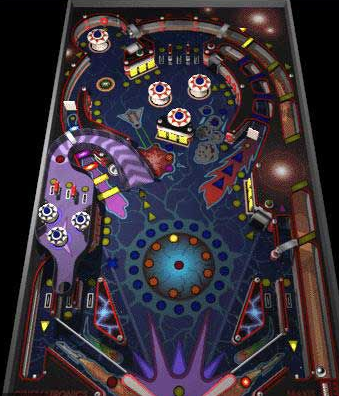
\includegraphics[width=0.3\linewidth]{coverimage1}\hfill
	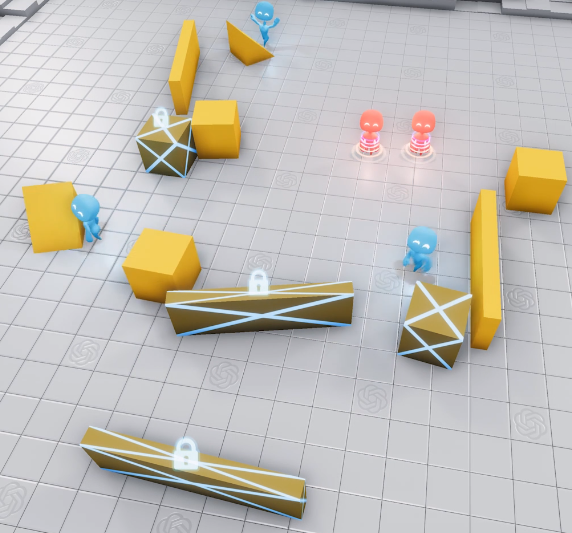
\includegraphics[width=0.3\linewidth]{OpenAI_cover}
\end{center}
\vspace{0.8cm}
% Author and supervisor
\noindent
\begin{minipage}{0.4\textwidth}
  \begin{flushleft} \large
    \emph{Authors :}\\
    Matthieu \textbf{{Thomas}}\\
    Julien \textbf{{Huynh}}\\
  \end{flushleft}
\end{minipage}%
\begin{minipage}{0.4\textwidth}
  \begin{flushright} \large
    \emph{Supervised by :} \\
    Mme \textbf{Frontera-Pons}\\
  \end{flushright}
\end{minipage}

\vfill

% Bottom of the page
{\large Version 0.1\\ \today}

\end{center}
\end{titlepage}

%%%%%%%%%%%%%%%%%%%%%%%%%%%%%
%%% Non-significant pages %%%
%%%%%%%%%%%%%%%%%%%%%%%%%%%%%

\frontmatter

%\chapter*{Remerciements}


\tableofcontents

\mainmatter
\pagestyle{fancy}
%%%%%%%%%%%%%%%%%%%%%%%%%%%%%%%%%%%%%%%%%%%%
%%% Content of the report and references %%%
%%%%%%%%%%%%%%%%%%%%%%%%%%%%%%%%%%%%%%%%%%%%
\chapter{Reinforcement learning}
\section{Why reinforcement learning ?}
\qquad While thinking about the way to use Machine Learning to play games, we thought of various possibilities but the one that stood out from the rest which is also the one used in many of those projects was reinforcement learning. The advantage of this method is that it works well when there are various states through time which is the case in games, for example, where the character is, what's its current status, its surroundings at a given time and much more. 
\section{Basics of reinforcement learning}
\subsection{Concepts}
\qquad Simply put, reinforcement learning is a method that takes advantage of the interactions between : 
\begin{itemize}
	\item Agent
	\item Actions
	\item Rewarding system
	\item Environment
	\item States
	\item Policy
	\item Value
\end{itemize}

Other concepts are also used but the ones mentioned above are the most essential ones.\\
\subsection{Main idea}
In reinforcement learning methods, the agent does a set of actions in order to maximize the reward it will get. At each given time, the agent will compute an action being given the state and this will then have a reaction from the environment surrounding it as a feedback which is the reward and will put it in a new state.\\

One representation of some of those interactions is the following loop :
\begin{figure}[H]
	\centering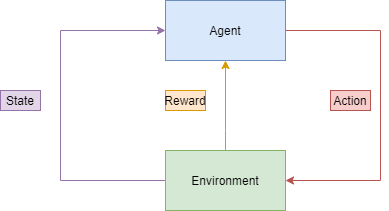
\includegraphics[width=0.6\linewidth]{RLSchema}
	\caption{Reinforcement learning concept interactions}
\end{figure}

On this loop, at a given time $t$, the agent knows the state $s_t$ and the reward $r_t$ at time $t$ and then computes an action $a_t$ with respect to $s_t$ and $r_t$. Then, the environment will give a new state $s_{t+1}$ and a new reward $r_{t+1}$ as a response to $a_t$. Obviously, the better the action taken was with respect to the objective, the higher the reward will be.\\

While it is debatable, reinforcement learning does not exactly fall into Supervised or Unsupervised learning because when the agent does the action, there are no labels. However, we could consider the reward as a time delayed label.
\subsection{Policy, Value and Trajectory}
While they did not appear in the loop, the trajectory, policy and value are essential in reinforcement learning.\\
\subsubsection{Policy}
\qquad The policy is the strategy the agent will use to reach its objective. If we refer to path-finding, it could be the different ways to go from a starting point to the objective point using different algorithms (Dijkstra, A$^*$, RRT, potential field, ...). Simply put, it defines how the agent will choose its action to have an impact on the environment. \\

The learning part is done at the \textbf{Agent} part which, given the state and the previous reward, will learn the best policy to maximize the value.
\subsubsection{Value}
\qquad In reinforcement learning, the value is basically the long term reward, it is what we would expect as an overall reward while being in a certain state and following a certain policy. The difference with the reward is that the latter is instantaneous, meaning that it is simply a response at a given time while the value is a much more global concept. Mathematically, it is defined as :
$$
V(s)=\mathbb{E}\left[\sum_{n}\gamma^n r_n\right]
$$

With $n$ the states, $r_n$ the reward for the state and $\gamma\in[0,1]$ a kind of damping factor for the reward, called discount factor. This factor helps giving a balance in the importance between the current reward and the ones to be expected in the "future". This is important in some situations when for example, an action is taken, giving a high reward at the given time but will also greatly reduce the expected future rewards thus, the value.
\subsubsection{Trajectory}
\qquad Roughly speaking, the trajectory $\tau$ is the set of states the agent went through after interacting with the environment.
\section{Model-based vs model-free}
One of the two important separations that we will see in Reinforcement learning is model-based versus model-free.\\

 Model-based algorithms learn a model meaning that they rely on states, actions and the \textbf{environment}. This means that if after the learning, our agent can predict the next state and reward related to it before even doing the action, it is a model-based algorithm. Those algorithms approximate a model of the environment. \\

On the other hand, model-free algorithms rely only on the states and the actions. They can \textbf{not} predict what the model-based algorithms can. The best action is not chosen using the environment. Those are "explicit" trial-and-error algorithms which are done using different methods such as the Monte Carlo method or temporal difference learning for example. One of the most popular reinforcement learning algorithms is Q-learning which is a model-free, off-policy algorithm.
\section{Q-Learning}
\qquad We choose to take a closer look at Q-Learning as it is one of the most popular reinforcement learning algorithms. Its objective is to maximize a value called the Q-value which is similar to the previously mentioned value but also takes the current action as an additional parameter.\\

An appropriate description for this $Q$ value would be quality of that given action and that would then allow us to estimate the score at the end without knowing what will come right after that given action (because we're model-free).\\

Obviously different actions will give different Q-values so in order to maximize our result, all we have to do is to choose the action that will give the highest Q-value. This implies learning the function, the mapping from the action to the Q-value and this process is Q-learning. This is done by saving and updating values in tables while approximating on the trial-and-error approach through the learning process.\\

While a basic Q-learning algorithm will do well on relatively small problems, issues will start rising once we approach bigger problems with more sophisticated and complex problems. This is especially true in our case with games where the actions can be limited in some very specific cases (PinBall or tic-tac-toe for example) but are in most games, very large, just like the number of states. Needless to say, such a large amount of data to store and update is inefficient and requires a huge computational power thus, the need for a more efficient technique.
\section{Deep reinforcement learning}
\qquad Deep reinforcement learning is a solution to our previously stated problem. As we mentioned, updating values and storing them is costly so we can try to approximate the function of this Q-value using Deep Neural Networks. As mentioned during our class, there is this fundamental theorem saying that Neural Networks can approximate about any function given the right number of neurons and layers. Thus, we could approximate the Q-value for each possible action given the state. This combination of learning a Q-function with a Deep Neural Network is called a Deep Q-Network (DQN)\\
\clearpage
With DQNs, the entry layer corresponds to the state (pixels for example) and the last layer is the different Q-values, one for each possible action. The so called labels used for propagation in this case is the targeted Q-values which can be computed from the Bellman Equation :

$$
Q_{target} (s_t,\ a_t)=\mathbb{E}\left[ r_{t+1}+\gamma \max_{a^{'}} Q_{target}(s^{'},\ a^{'}) \right] 
$$

We could then consider the loss as a comparison between this targeted Q-value and the resulting output of our network and then tune as we would do with any typical neural network.\\

\begin{figure}[H]
	\centering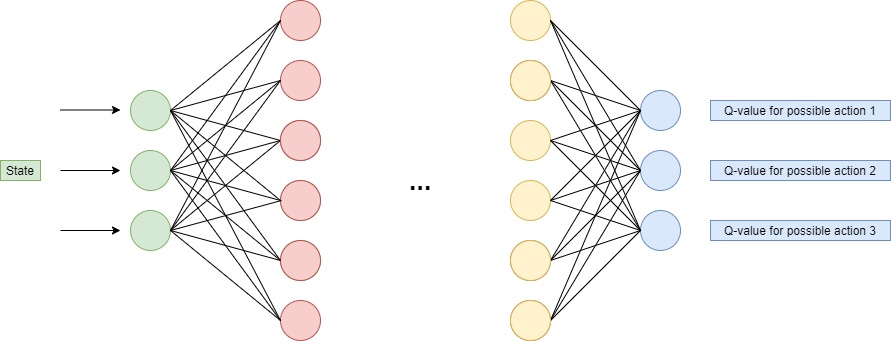
\includegraphics[width=\linewidth]{DQN}
	\caption{Deep Q Network input/output}
\end{figure}

The idea behind this is still to solve the same problem as with Q-Learning but with a different method to make it more efficient.\\

As the number of Machine Learning and game enthusiasts increase online so do the number of projects linking those two domains and, in many of those projects, this particular reinforcement learning method is used, especially since the reawakening of Deep Neural Networks over the last years with the increasing computation powers we have at our disposal.


\chapter{Reinforcement learning - Examples of applications}
\section{3D PinBall AI}
\qquad While searching a subject for this project, we came across the idea that we could use reinforcement for a game with few inputs to have an easy decision making. We found quickly this project made by Elliot Wood, we wanted to try it out but the installation methods aren't on point. The objective of the AI is to gain score as fast as possible without supervision. We originally wanted to center the project around this application but we couldn't manage to execute training sessions on the game. The inputs are very limited, right and left triggers, the agents understand with ease that they must not let the ball pass by a trigger without sending it up else they lose a life and get punished. They also save the patterns where they gain a lot of points to be able to reproduce it as well. This example is an approach of reinforcement learning used to train intelligent agents in video games. 

\section{Open AI : Multi agents hide and seek}
\qquad This fun co-op game created by OpenAI, a research laboratory based in San Francisco is the opportunity to let agents show their creativity. The 2 teams are seekers and hiders, the goal of seekers is to have in line of sight the hiders, the goal of hiders is to survive for long enough. They get rewarded based on the time they can survive or find the hiders. Both teams can move around and push/pull the yellow blocks but the hiders team can lock blocks and they can't be moved by the seekers. For the first training level, the hiders team agents could only win through cooperation by blocking the 2 doors and stay inside the room. They started by running errands, then the seekers started to follow the hiders pretty quickly, it took the hiders 2.69 millions of games to understand how to block the doors at the beginning of the round. We can see at the top right corner we can see a ramp that will be used by the seekers to climb above the wall of the room from the 8.62 million game to the game number 14.5 million. The hiders started to win again at this time by taking the ramp inside the room with them before locking themselves with it. The level was designed by the researchers to show the evolution through times and tries that these agents could have. The researchers, hope that their discoveries will be useful for other applications in the industry. 


\begin{figure}[H]
	\centering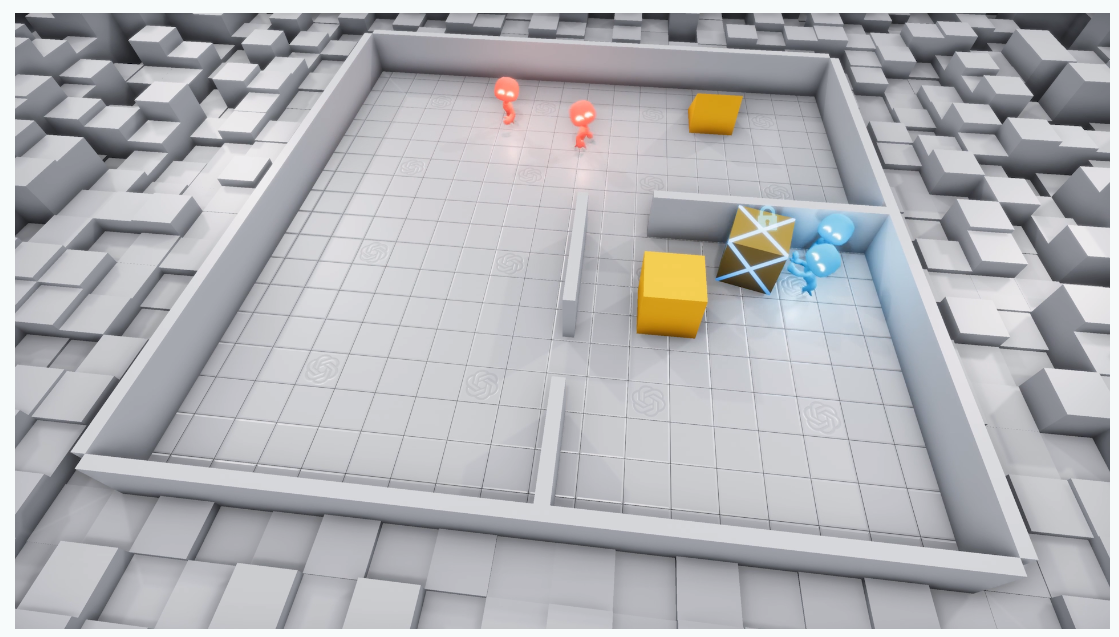
\includegraphics[width=\linewidth]{OpenAI1.png}
	\caption{First training environment}
\end{figure}

\qquad This other environment allowed more and more creativity for the agents, the hiders first tried to create a wall and lock themselves in, it worked and they were rewarded for their win until the seekers agents discovered they could go over the wall with the ramps. The next move of the hiders was to lock the ramp away from their defense, they kept on winning for a long time until the seekers exploited a bug they found ! They move a box square close to a ramp and climb on the box by using the ramp, while on top of the box there is a bug that the developers didn't think of at first but they could move the box with themselves on top ! So they had the ability to move freely around and go over the hiders walls. The hiders then locked the ramps AND the boxes so that this bug couldn't be exploited anymore by the seekers and won all rounds.

\begin{figure}[H]
	\centering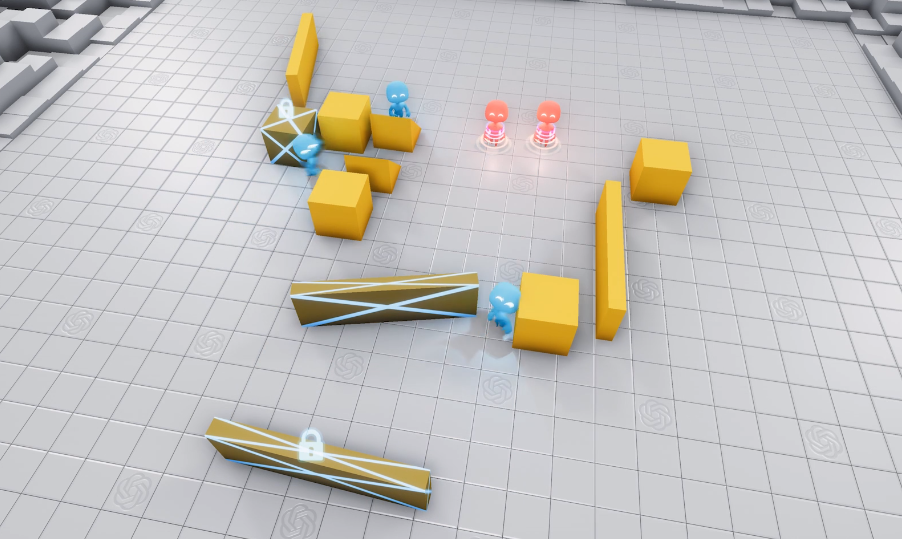
\includegraphics[width=\linewidth]{OpenAI2.png}
	\caption{Open training environment}
\end{figure}

\section{StarCraft 2 Agents : AlphaStar}
\qquad StarCraft is one of the most complete RTS (Real Time Strategy) game on the market. This is why the result obtained by the AlphaStar agents are impressive, they are reinforced agents trained against each other, that made it to the top level of the global ladder (best 0.02\% of the active players) and beat the current world best players during a show-match. While playing, the agent sees the same thing as a player sees on a screen and has a number of moves per minute limited, APMs (actions per minute) is a factor that can cleave players so AlphaStar APMs were nerfed and limited to something humans can reach. The way it was trained was first copying mechanisms, then self play against others agents and remembering what makes an agent wins, then specific decisions based on pro games, then really advanced AIs were trained to react to specific strategies made by abusers agents. The agents were playing in ranked matches all along the training and there is a quick video showing how far they could go with each method of training (see below). The pro players that played against these AIs said that they were playing perfectly, but not on an inhuman level, it would be theoretically possible to reach by a human player but the consistency would not match AlphaStar perfect game-play. 

\url{https://www.youtube.com/watch?v=xP7LwZxq0ss&feature=emb_title}

\clearpage
\chapter*{Sources}
\begin{itemize}
	\footnotesize
	\item\url{https://towardsdatascience.com/simple-reinforcement-learning-q-learning-fcddc4b6fe56}
	\item\url{https://www.freecodecamp.org/news/an-introduction-to-q-learning-reinforcement-learning-14ac0b4493cc/}
	\item\url{https://www.geeksforgeeks.org/what-is-reinforcement-learning/}
	\item\url{https://www.kdnuggets.com/2018/03/5-things-reinforcement-learning.html}
	\item\url{https://towardsdatascience.com/keras-transfer-learning-for-beginners-6c9b8b7143e}
	\item\url{https://pathmind.com/wiki/deep-reinforcement-learning}
	\item\url{https://deepmind.com/blog/article/AlphaStar-Grandmaster-level-in-StarCraft-II-using-multi-agent-reinforcement-learning}
	\item\url{https://unitylist.com/p/w1g/3D-Pinball-AI}
	\item\url{https://openai.com/blog/emergent-tool-use/}
    \item Various online courses/videos 
    
\end{itemize}
\end{document}